\documentclass[10pt,twocolumn,letterpaper]{article}

\usepackage{times}
\usepackage{graphicx}
\usepackage{amsmath}
\usepackage{amssymb}
\usepackage{booktabs}
\usepackage{multirow}
\usepackage{url}
\usepackage[breaklinks=true,letterpaper=true,colorlinks,citecolor=blue,bookmarks=false]{hyperref}

\def\cvprpaperID{**} % Placeholder per eventuale ID corso
\def\httilde{\mbox{\tt\raisebox{-.5ex}{\symbol{126}}}}
\usepackage{xcolor}
\definecolor{arXiv}{HTML}{B31B1B}
\usepackage[backend=biber, style=numeric,maxnames=99]{biblatex}
\addbibresource{biblio.bib}
\begin{document}

%%%%%%%%% TITLE
\title{Comprehensive Road Scene Understanding for Autonomous Driving}



\author{
Andrea Nardo \hspace{1cm}
Flavio Frasca \hspace{1cm}
Francesca Longo \hspace{1cm}
Giuditta Macigno
}

\date{}

\maketitle

\begin{abstract}
Semantic segmentation is a fundamental component of autonomous driving systems, but most existing approaches are designed under a closed-set assumption and often struggle when unexpected objects appear in the scene. In this project, we investigate the use of the Encoder-only Mask Transformer (EoMT) for joint semantic segmentation and anomaly detection in urban driving environments.

Starting from a COCO-pretrained model, we adapt EoMT to Cityscapes through a label remapping strategy and a Layer-wise Learning Rate Decay (LLRD) fine-tuning procedure. We compare the original COCO model, a Cityscapes-trained version, and our fine-tuned model against the pixel-based ERFNet baseline.

Experiments on Cityscapes, SMIYC, and Fishyscapes show that fine-tuning significantly improves semantic segmentation performance while preserving the benefits of mask-based representations for anomaly localization. In particular, region-level anomaly scoring methods produce more coherent anomaly maps and more accurate localization of out-of-distribution objects than conventional pixel-wise uncertainty measures. [GitHub repository: \url{https://github.com/flaviofrasca/MaskArchitectureAnomaly_CourseProject}]
\end{abstract}
\begin{figure*}[t]
    \centering
    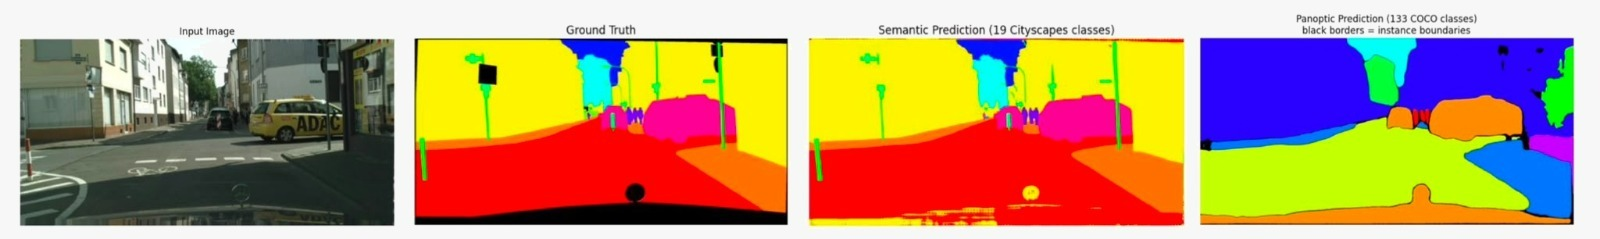
\includegraphics[width=\textwidth]{image.jpeg}
    \caption{Qualitative results of the EoMT model on a Cityscapes validation sample. From left to right: input image, ground-truth semantic annotation, semantic segmentation prediction on the 19 Cityscapes classes, and the corresponding panoptic prediction in the original 133-class COCO taxonomy remapped to Cityscapes calsses. The example illustrates how the model preserves rich open-world representations while producing accurate semantic segmentation in urban driving scenarios.}
    \label{fig:qualitative_results}
\end{figure*}

\section{Introduction}

Semantic segmentation plays a central role in autonomous driving by providing a dense understanding of the environment and enabling vehicles to distinguish between roads, vehicles, pedestrians, and other relevant scene elements. Although significant progress has been achieved, most segmentation models are still trained under a closed-set assumption, forcing every pixel to belong to one of the classes seen during training. In real-world scenarios, however, unexpected objects may appear, often leading models to produce overconfident predictions for unknown regions.

Traditional architectures such as ERFNet formulate semantic segmentation as a pixel-level classification task, assigning labels independently to each image location. While efficient, this approach does not explicitly capture object structure and can produce fragmented predictions, especially around boundaries or in visually complex scenes.

More recent methods adopt mask-based representations, an evolution partly driven by panoptic segmentation, which unifies semantic and instance segmentation. Architectures such as MaskFormer and Mask2Former predict object masks and class labels through a set of learned queries. The Encoder-only Mask Transformer (EoMT) follows this paradigm while leveraging large-scale pre-trained visual representations.

Beyond semantic segmentation, we focus on anomaly detection, where the objective is to identify regions that do not belong to the categories observed during training. Rather than modifying the training procedure, we investigate post-hoc anomaly scoring methods that can be applied directly to model outputs and evaluate their effectiveness on standard anomaly segmentation benchmarks.


\section{Methodology}

\textbf{Problem Formulation and Architectures}
To study how architectural design affects anomaly detection, we consider models with different structures and training setups. ERFNet is a convolutional pixel-level classifier trained on Cityscapes, producing per-pixel class probabilities over 19 categories. EoMT, instead, is a transformer-based model, which predicts segmentation through a set of masks rather than direct pixel-wise classification. In our experiments, we consider three versions of EoMT: one used directly after COCO pre-training, one fine-tuned on Cityscapes and one directly trained on Cityscapes.

Because of these differences, a direct comparison is not straightforward. ERFNet and EoMT trained directly on Cityscapes can be evaluated directly since they already operate in the right label space. The COCO-pretrained EoMT requires additional steps, including a taxonomy mapping from COCO to Cityscapes and further adaptation to the target domain through fine-tuning.

\textbf{Cross-Dataset Taxonomy Alignment.}
A foundational challenge in adapting the COCO-pretrained model to our task is the label space mismatch between the pre-training domain and the target domain: COCO defines 133 categories, while Cityscapes uses 19 classes. To run zero-shot evaluation, we implemented a dense remapping tensor (\texttt{COCO\_TO\_CITYSCAPES}), initialized entirely to the ignore index ($255$) and then populated according to three rules: categories with an exact match are directly mapped to the corresponding Cityscapes class, similar categories are grouped into the closest semantic class and all remaining categories are assigned to the ignore index ($255$).
This mapping is only used for zero-shot evaluation. During fine-tuning, the classification head is replaced and the model is trained directly on Cityscapes labels without any remapping.

\textbf{Parameter-Efficient Fine-Tuning via LLRD.}
Our training setup follows a transfer learning strategy, where a COCO-pretrained model is fine-tuned on Cityscapes using Layer-wise Learning Rate Decay (LLRD). We choose LLRD instead of adapter methods like LoRA because it allows full-network fine-tuning without introducing additional parameters, keeping the model architecture unchanged and computationally efficient.

Instead of explicitly freezing and unfreezing parts of the network, LLRD keeps the entire model trainable and control the adaptation through layer-dependent learning rates. In this way, lower layers are updated more conservatively while higher layers adapt more strongly to the target domain. This avoids damaging low-level representations learned during pre-training while still allowing effective domain adaptation.

The classification and mask heads are trained with the full learning rate throughout the process.

Training is divided into four phases. In the first phase (10 epochs), we freeze the entire backbone (\texttt{lr\_mult} $= 0.0$) and train only the task-specific heads to stabilize the optimization. In the following phases, we progressively unfreeze the model and apply Layer-wise Learning Rate Decay with $\gamma = 0.3$, $0.6$, and $0.8$, each for 5 epochs.

In practice, $\gamma = 0.6$ gives the best trade-off, reaching 79.8\% mIoU, while $\gamma = 0.8$ slightly degrades performance to 79.3\%, suggesting that too much adaptation of early layers can harm the pre-trained representations. 

\textbf{Post-hoc Anomaly Scoring.}
To extract pixel-wise anomaly maps, we apply three post-hoc scoring methods to all models: Maximum Softmax Probability (MSP), MaxLogit, and MaxEntropy. Additionally, Rejected by All (RbA) is evaluated exclusively on the mask-based EoMT architectures, as it requires query-level mask representations unavailable in pixel-level classifiers. Instead of looking for anomalies pixel by pixel, RbA evaluates entire spatial regions. It aggregates evidential values from the mask queries and assigns a single anomaly score based on the overall uncertainty of that specific area. Efficacy is evaluated directly using threshold-free metrics (AuPRC and FPR95).

To investigate whether confidence calibration could improve anomaly detection, we also apply Temperature Scaling to MSP, which is often affected by overconfident predictions. By adjusting the softmax temperature, this method modifies the confidence distribution without changing the predicted classes, allowing us to evaluate the impact of calibration on anomaly scoring.

\section{Experimental Results}

\textbf{Datasets and Evaluation Protocol.}
The empirical evaluation is divided into two main tasks: closed-set semantic segmentation and open-world anomaly segmentation. For the first evaluation, we use the validation split of the Cityscapes dataset, which contains urban driving images annotated across 19 target categories. To assess out-of-distribution generalization, we benchmark on the SegmentMeIfYouCan (SMIYC) dataset (RoadAnomaly21 and RoadObstacle21 tracks),the Fishyscapes benchmark (Lost and Found and Static subsets) and the Road Anomaly dataset. For EoMT models, pixel-wise logits are extracted directly from the mask queries via the \texttt{to\_per\_pixel\_logits} semantic function, bypassing standard panoptic post-processing heuristics (e.g., Non-Maximum Suppression). Model performance is quantified using the Mean Intersection over Union (mIoU) for semantic segmentation, and the Area Under the Precision-Recall Curve (AuPRC) alongside the False Positive Rate at 95\% True Positive Rate (FPR95) for anomaly segmentation.

\textbf{Quantitative Results.}
Table~\ref{tab:miou_results} reports the performance of the models on 
semantic segmentation over the Cityscapes validation set. The Cityscapes 
pre-trained baseline establishes the architectural upper bound at 81.7\% 
mIoU, while EoMT COCO, through our class mapping strategy, obtains a 
mIoU of 55.1\%. Our fine-tuned model reaches 79.8\% mIoU, whereas 
ERFNet yields 72.2\% mIoU as the pixel-level baseline.

\begin{table}[h]
\caption{Semantic Segmentation Performance (mIoU) on the Cityscapes Validation Set.}
\label{tab:miou_results}
\begin{center}
\resizebox{\columnwidth}{!}{
\begin{tabular}{lcl}
\toprule
\textbf{Model Configuration} & \textbf{mIoU (\%)} & \textbf{Key Characteristics} \\
\midrule
ERFNet (Pixel Baseline) & 72.2 & Standard convolutional architecture \\
EoMT COCO (Zero-Shot) & 55.1 & Taxonomy mapping \\
EoMT Fine-Tuned (Ours) & 79.8 & LLRD adaptation ($\gamma=0.6$) \\
EoMT Cityscapes (Orig.) & 81.7 & Upper-bound baseline \\
\bottomrule
\end{tabular}
}
\end{center}
\end{table}

Table~\ref{tab:anomaly_results} presents the anomaly segmentation results. 
For ERFNet, MaxLogit obtains the highest scores, attaining 38.32 AuPRC 
and 59.34 FPR95 on SMIYC RA-21, and 15.58 AuPRC and 73.25 FPR95 
on Road Anomaly. For EoMT COCO, all scoring methods produce 
consistently low AuPRC values across all benchmarks. For EoMT 
Cityscapes, MaxEntropy achieves 90.00 AuPRC on SMIYC RO-21, while 
RbA attains 90.25 AuPRC on the same benchmark. For our fine-tuned 
model, RbA reaches 94.00 AuPRC and 0.43 FPR95 on SMIYC RO-21, 
and 85.18 AuPRC and 5.50 FPR95 on FS Static.

Table~\ref{tab:tempscaling} reports the results of Temperature Scaling applied to the MSP scoring method across all three EoMT checkpoints. The optimal temperature $T^\star$ is 2.00 for the majority of benchmarks. Across all models and datasets, the maximum observed AuPRC improvement is $+0.14$, while several configurations yield no measurable change ($\Delta = 0.00$).

\begin{table*}[t]
\caption{Anomaly Segmentation Performance (AuPRC $\uparrow$ / FPR95 $\downarrow$) on SMIYC, Fishyscapes, and RoadAnomaly benchmarks.}
\label{tab:anomaly_results}
\begin{center}
\resizebox{\textwidth}{!}{
\begin{tabular}{llc|cc|cc|c}
\toprule
\textbf{Model} & \textbf{Cityscapes mIoU} & \textbf{Scoring Method} & \textbf{SMIYC RA-21} & \textbf{SMIYC RO-21} & \textbf{FS Static} & \textbf{FS L\&F} & \textbf{Road Anomaly} \\
\midrule
\multirow{3}{*}{ERFNet} 
& \multirow{3}{*}{72.2\%} 
& MSP & 29.10 / 62.55 & 2.71 / 65.22 & 7.47 / 41.84 & 1.75 / 50.59 & 12.42 / 82.58 \\
& & MaxLogit & \textbf{38.32} / \textbf{59.34} & 4.63 / 48.44 & 9.50 / 40.30 & 3.30 / 45.49 & \textbf{15.58} / \textbf{73.25} \\
& & MaxEntropy & 30.97 / 62.66 & 3.04 / 65.91 & 8.84 / 41.55 & 2.58 / 50.16 & 12.67 / 82.75 \\
\midrule
\multirow{4}{*}{EoMT (COCO)} 
& \multirow{4}{*}{55.1\%} 
& MSP & 38.88 / 77.50 & 2.76 / 99.98 & 4.67 / 99.48 & 3.78 / 97.21 & 18.86 / 91.84 \\
& & MaxLogit & 39.37 / 77.00 & 2.76 / 99.98 & 4.70 / 99.46 & 3.78 / 97.21 & 19.03 / 91.58 \\
& & MaxEntropy & 43.26 / 63.32 & 8.35 / 99.98 & 4.57 / 99.32 & 3.78 / 96.93 & 21.54 / 87.88 \\
& & RbA & 24.78 / 89.18 & 3.16 / 100.00 & 3.01 / 99.55 & 2.92 / 52.28 & 18.19 / 94.42 \\
\midrule
\multirow{4}{*}{EoMT (Cityscapes)} 
& \multirow{4}{*}{81.7\%} 
& MSP & 66.08 / 34.33 & 89.85 / 0.33 & 62.50 / 28.09 & 17.58 / 20.69 & 66.90 / 19.89 \\
& & MaxLogit & 65.96 / 34.68 & 89.84 / 0.33 & 62.49 / 29.11 & 17.58 / 20.46 & 66.47 / 19.78 \\
& & MaxEntropy & 69.11 / 34.17 & \textbf{90.00} / 0.32 & 60.46 / 28.38 & 19.61 / 20.58 & 70.17 / 19.39 \\
& & RbA & 66.07 / 38.12 & 90.25 / 0.32 & \textbf{62.06 / 28.88} & 17.69 / 20.34 & \textbf{66.26} / 19.48 \\
\midrule
\multirow{4}{*}{EoMT (Fine-Tuned)} 
& \multirow{4}{*}{79.8\%} 
& MSP & 66.98 / 30.12 & 92.61 / 0.53 & 86.06 / 5.66 & 29.44 / 21.51 & 52.57 / 26.26 \\
& & MaxLogit & 66.89 / 29.65 & 92.52 / 0.54 & \textbf{86.07 / 5.38} & 29.61 / 20.65 & 52.41 / 25.88 \\
& & MaxEntropy & 68.67 / 29.45 & \textbf{92.50} / 0.54 & 85.73 / 4.89 & 31.71 / 20.59 & 53.70 / 25.53 \\
& & RbA & 60.99 / 34.48 & 94.00 / 0.43 & 85.18 / 5.50 & 29.64 / 21.55 & \textbf{51.89} / 25.55 \\
\bottomrule
\end{tabular}
}
\end{center}
\end{table*}


\section{Discussion}

\textbf{Semantic Segmentation: Model Comparison.}
The evaluation on Cityscapes of our COCO pre-trained baseline clearly shows an interesting behaviour of the model. A detailed per-class analysis demonstrates how the model performs strongly on simple and common elements, reaching 94.1\% IoU on \textbf{road} (a marginal drop of $-4.3$ percentage points compared to the Cityscapes upper bound), 89.7\% on \textbf{sky} and 87.7\% on \textbf{vegetation}. Conversely, a gap of 26.6 percentage points between the mapped COCO model and the Cityscapes baseline highlights two fundamental issues.

\begin{enumerate}
    \item \textbf{Absolute Taxonomic Voids}: the drop is heavily influenced by classes completely absent from COCO's taxonomy. For instance, \textit{pole} and \textit{rider} achieve exactly 0.0\% IoU, while \textit{traffic sign} is limited to a mere 4.7\% (a dramatic drop of $-77.4$ pp).

    \item \textbf{Morphological Domain Shifts}: while standard cars maintain a robust 84.3\% IoU, heavily articulated European urban vehicles differ significantly from general open-world distributions, causing severe misclassifications for \textit{truck} (29.4\%, $\Delta = -52.4$) and \textit{train} (13.6\%, $\Delta = -63.7$).
\end{enumerate}

By fine-tuning the model on Cityscapes via LLRD we successfully dismantle these bottlenecks. The fine-tuning reconstructs the missing taxonomic concepts (\textit{pole} recovers to 66.4\% and \textit{traffic sign} to 79.9\%). As shown in Table ~\ref{tab:perclass}, the fine-tuned model surpasses the Cityscapes baseline for morphologically complex classes, reaching 84.1\% on \textit{train} (vs 77.4\%) and 82.5\% on \textit{truck} (vs 81.8\%). This demonstrates that the COCO prior, once properly aligned, provides a richer feature representation for complex objects compared to training on narrow urban datasets alone.
Regarding ERFNet, the pixel-level baseline achieves 72.2\% mIoU, 
confirming its competitiveness despite being significantly simpler than mask-based models.

\begin{table}[t]
\centering
\caption{Temperature Scaling on MSP (AuPRC \%). For each model and benchmark we
report the baseline ($T{=}1$), the best value found via grid search over
$T \in [0.1, 2.0]$, the optimal temperature $T^\star$, and the resulting gain
$\Delta$.}
\label{tab:tempscaling}
\scriptsize
\setlength{\tabcolsep}{2.5pt}
\resizebox{\columnwidth}{!}{
\begin{tabular}{llcccc}
\toprule
Model & Dataset & Base & Best & $T^\star$ & $\Delta$ \\
\midrule
\multirow{5}{*}{EoMT COCO}
  & SMIYC RA-21 & \textbf{38.87} & \textbf{38.98} & 2.00 & +0.11 \\
  & SMIYC RO-21 &  2.77 &  2.77 & 2.00 & +0.00 \\
  & FS L\&F     &  3.80 &  3.81 & 2.00 & +0.01 \\
  & FS Static   &  4.70 &  4.71 & 1.85 & +0.01 \\
  & Road Anom.  & 18.89 & 18.92 & 2.00 & +0.03 \\
\midrule
\multirow{5}{*}{EoMT Cityscapes}
  & SMIYC RA-21 & \textbf{66.83} & \textbf{66.97} & 2.00 & \textbf{+0.14} \\
  & SMIYC RO-21 & 89.90 & 89.90 & 2.00 & +0.00 \\
  & FS L\&F     & 18.22 & 18.24 & 2.00 & +0.02 \\
  & FS Static   & 63.47 & 63.47 & 1.40 & +0.00 \\
  & Road Anom.  & 67.78 & 67.92 & 2.00 & +0.14 \\
\midrule
\multirow{5}{*}{EoMT Fine-Tuned}
  & SMIYC RA-21 & \textbf{67.48} & \textbf{67.54} & 1.90 & +0.06 \\
  & SMIYC RO-21 & 92.65 & 92.70 & 0.10 & +0.05 \\
  & FS L\&F     & 30.45 & 30.46 & 2.00 & +0.01 \\
  & FS Static   & 86.28 & 86.29 & 2.00 & +0.01 \\
  & Road Anom.  & 52.98 & 52.99 & 2.00 & +0.01 \\
\bottomrule
\end{tabular}
}
\end{table}

\textbf{Anomaly Segmentation and Scoring.}
The anomaly detection results reveal the importance of the training domain. As shown in Table~\ref{tab:anomaly_results}, the zero-shot EoMT COCO model fails across all anomaly benchmarks, exhibiting FPR95 values close to 100\% in most cases. This behaviour is expected, as a model trained exclusively on the COCO taxonomy lacks a clear notion of road-scene semantics. Consequently, anomaly scores become largely uninformative and fail to discriminate between in-distribution and out-of-distribution regions. Fine-tuning with LLRD dramatically changes this picture: the EoMT FT model consistently outperforms ERFNet on all evaluated datasets, achieving, for instance, an AuPRC of 92.50\% on SMIYC RO-21.

A comparison between the fine-tuned model and the Cityscapes-pretrained EoMT baseline reveals a more nuanced behaviour. On datasets characterized by clear physical obstacles appearing on the road surface, such as SMIYC RO-21 and Fishyscapes Static, the fine-tuned model provides substantial improvements. On Fishyscapes Static, for example, AuPRC increases from 62.06\% to 86.07\%, while FPR95 decreases from 28.88\% to 5.38\%. This suggests that fine-tuning enables the model to improve its ability to identify objects that do not belong to the drivable area. However, this specialization comes at a cost. On the Road Anomaly benchmark, the fine-tuned model performs approximately 16 percentage points worse than the Cityscapes-pretrained baseline. This indicates that the adaptation process increases sensitivity to urban environments while reducing robustness to rare or rural anomalies not represented during fine-tuning.

Regarding the anomaly scoring strategies, Temperature Scaling was investigated to determine whether calibration could improve the performance of Maximum Softmax Probability (MSP). In practice, however, the impact is negligible. On SMIYC RA-21, the optimal temperature modifies the AuPRC of the COCO model only from 38.87\% to 38.98\%, the Cityscapes model from 66.83\% to 66.97\%, and the fine-tuned model from 67.48\% to 67.54\%. These results suggest that the limitations of MSP are not primarily related to calibration. Since MSP relies exclusively on the highest predicted probability, it ignores potentially informative uncertainty contained in the remaining distribution. Moreover, MaxEntropy, by considering the full probability distribution, provides a more reliable measure of model uncertainty and consistently achieves superior anomaly detection performance emerging as the most stable method across all evaluated checkpoints.

\section{Conclusion}

\begin{table}[t]
\centering
\caption{Per-class IoU (\%) on the Cityscapes validation set. EoMT~CS is the
fully specialized upper bound; EoMT~FT is our LLRD fine-tuned model.}
\label{tab:perclass}
\small
\setlength{\tabcolsep}{4pt}
\begin{tabular}{lcccc}
\toprule
Class & EoMT CS & EoMT COCO & EoMT FT & ERFNet \\
\midrule
road          & 98.4 & 94.1 & 98.3 & 97.6 \\
sidewalk      & 87.4 & 64.8 & 85.6 & 81.2 \\
building      & \textbf{94.1} & 87.1 & 93.6 & 90.8 \\
wall          & 66.1 & 46.0 & 60.0 & 49.5 \\
fence         & 65.5 & 49.8 & 59.7 & 54.9 \\
pole          & 71.0 &  \textbf{0.0} & \textbf{66.4} & 60.8 \\
traffic light & 75.0 & 60.6 & 73.1 & 62.6 \\
traffic sign  & 82.1 &  \textbf{4.7} & \textbf{79.9} & 72.2 \\
vegetation    & 93.0 & \textbf{87.7} & 93.0 & 91.4 \\
terrain       & 66.6 & 56.7 & 65.6 & 61.0 \\
sky           & 95.5 & \textbf{89.7} & 95.2 & 93.2 \\
person        & 85.4 & 70.5 & 85.1 & 76.2 \\
rider         & 71.1 &  \textbf{0.0} & 66.2 & 53.5 \\
car           & 95.5 & \textbf{84.3} & 95.3 & 92.8 \\
truck         & 81.8 & \textbf{29.4} & \textbf{82.5} & 72.7 \\
bus           & 90.3 & 71.2 & 88.3 & 78.8 \\
train         & 77.4 & 13.6 & \textbf{84.1} & 63.8 \\
motorcycle    & 74.4 & 63.8 & 65.0 & 46.4 \\
bicycle       & 81.3 & 73.3 & 80.2 & 71.9 \\
\midrule
mIoU          & 81.7 & 55.1 & 79.8 & 72.2 \\
\bottomrule
\end{tabular}
\end{table}

In this project, we evaluated EoMT for semantic segmentation and anomaly detection in autonomous driving scenarios. Our results show that adapting a COCO-pretrained model to Cityscapes significantly improves on both tasks, outperforming the ERFNet baseline on all evaluated anomaly benchmarks.

The experiments also highlight the importance of the training domain. While fine-tuning improves the detection of urban road obstacles, it can reduce generalization to anomaly types that are less represented during adaptation which could be further investigated in future work. Finally, among the scoring methods considered, MaxEntropy proved to be the most reliable.


\section*{Acknowledgments}
The authors declare that Generative AI tools were not used for writing this project report. 

Regarding the development of the submitted project code, Generative AI tools were utilized to assist the programming workflow in the following manner:
\begin{itemize}
    \item \textbf{Name and version:} Claude Code, Sonnet 4.6
    \item \textbf{Publisher:} Anthropic
    \item \textbf{Context and Usage:} The tool was employed strictly as a coding assistant to help troubleshoot syntax errors, format Python scripts, and optimize PyTorch tensor operations during the LLRD implementation. It was not used for experimental decision-making. All AI-generated suggestions were subjected to rigorous human supervision. Engineering judgment was constantly applied to manually verify, adapt, and integrate the snippets into the EoMT fine-tuning and evaluation pipelines, ensuring mathematical correctness and structural consistency with the evaluation protocol. 
\end{itemize}

All group members are jointly responsible for these declarations and guarantee that the use of such tools involved continuous review and strict human oversight throughout the entire experimental analysis process.

{\small
\nocite{*}
\printbibliography
}
\end{document}

